\documentclass[a4paper,10pt]{article}
\usepackage[utf8]{inputenc}
\usepackage{amsmath}
\usepackage{graphicx}

%opening
\title{Methods used}
\author{Bram van Es \& Sebastiaan Jong}

\begin{document}


\begin{abstract}

\end{abstract}


% Description of what is done
  % Detailed description of array normalization and batch correction strategy
  % Detailed description of procedures
  % Potential literature references
  % Flow charts
  % Thresholds/cut-offs
  % Iterations
  % Scripts (github), some journals require scripts
% In between results
  % Description of results obtained using your strategy and validation.
  % Plots/tables/text containing information of why this is a valid approach, for multiple steps
  % Rational behind the idea, prove of correctness
% Prediction of HR/NHR for ALL10
% Prediction of HR/NHR for Cohort1


\section{Pre-processing}

\subsection{Cohort-bias removal}
%
For the cohort-bias removal we apply a genome-wise Location and scale (L/S) adjustment per cohort.
Using a normalisation per cohort guarantees that the features have the same bounds 
over the cohorts and that the means are similar. The caveat of this approach is that we asume 
that the genome expression measurements are independent and we have no outliers.
%
The standard normalisation transforms the genome expression values $\mathbf{x}$ per genome as follows
\begin{equation}
  \mathbf{x}^* = \frac{\mathbf{x} - \overline{\mathbf{x}}}{\sigma},
\end{equation}
%
where $\mathbf{x}$ is the genome expression vector for some genome over all samples. 
This centers the mean and normalises the  expression values with the standard deviation. 
To limit the influence of outliers we can center the median and use the interquantile range (IQR)
for the scaling, i.e.
%
\begin{equation}
  \mathbf{x}^* = \frac{\mathbf{x} - median\left({\mathbf{x}}\right)}{IQR},
\end{equation}
%
%To ensure similar bounds we can then scale the values by largest absolute value per genome vector, i.e.
%\begin{equation}
%  \mathbf{x}^* = \frac{\mathbf{x}}{\max{(\mathbf{x})}}.
%\end{equation}
%
To demonstrate the effect of these transformations with regard to cohort bias we take two genomes, one with high and one with low variance
over the classifications. \\ \\
%
\begin{figure}[htp]
\centering
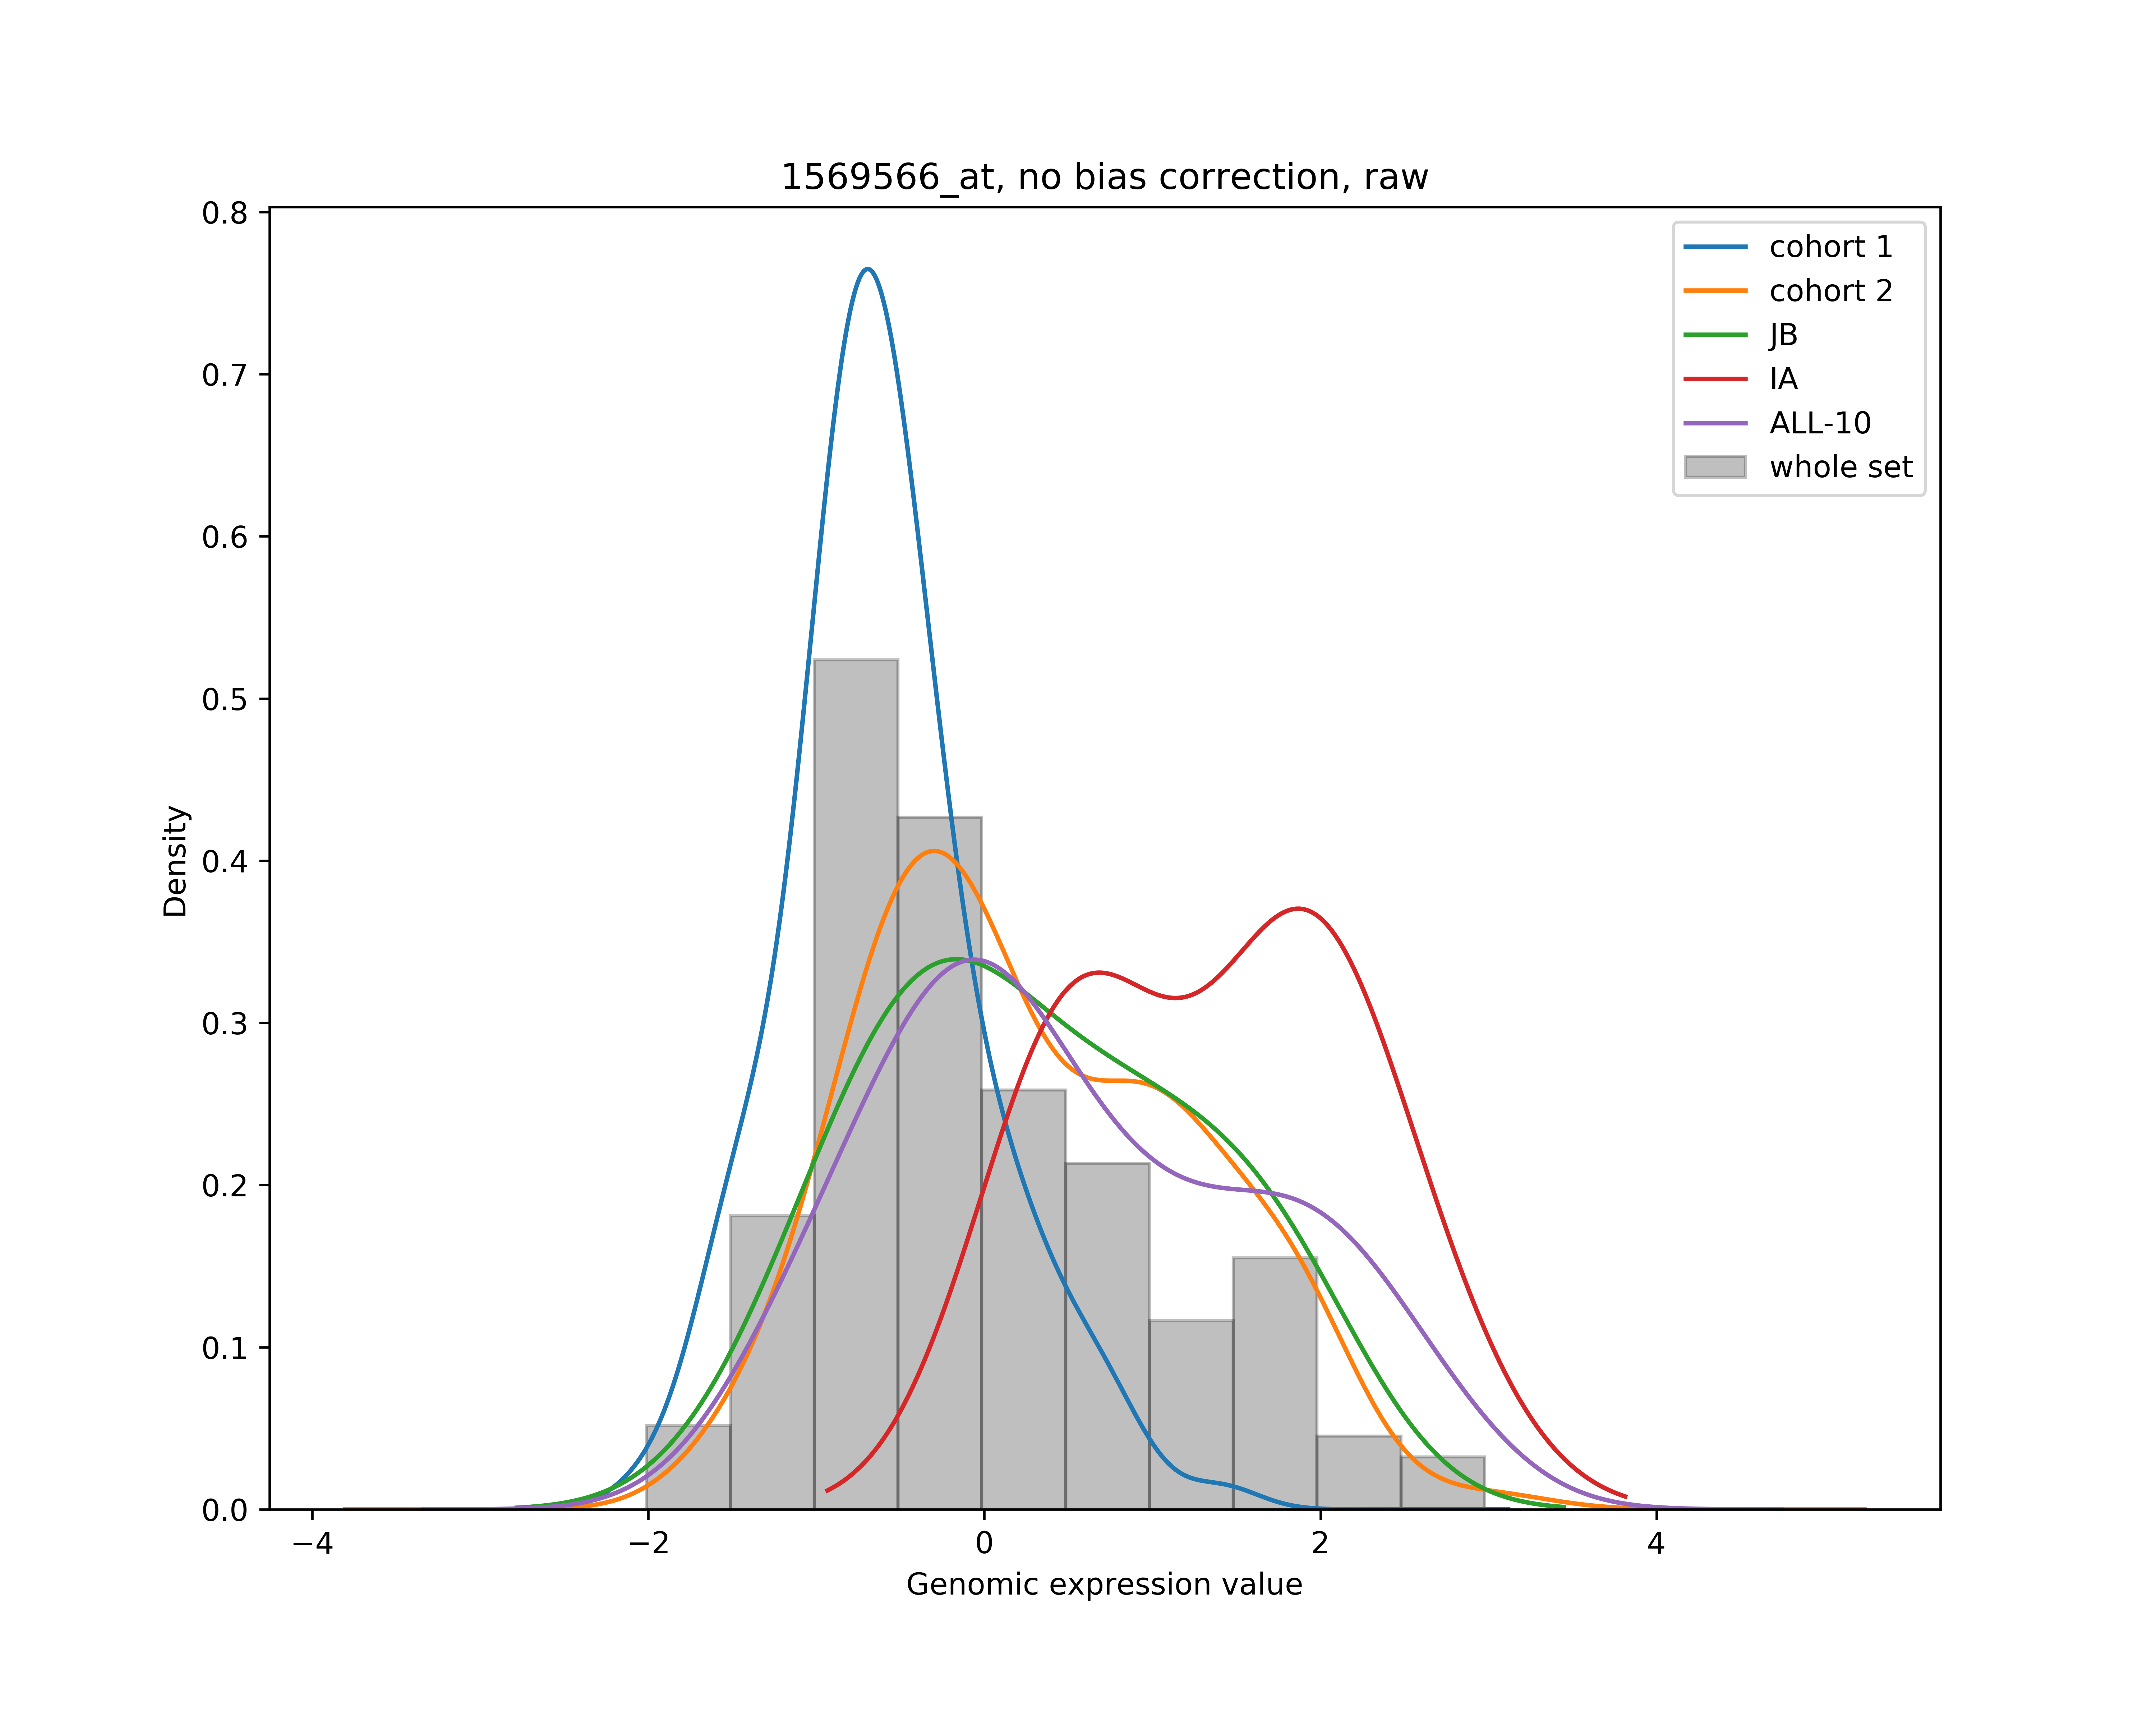
\includegraphics[width=6cm]{images/strong_genome_distribution_noCorrection_noNormalisation}
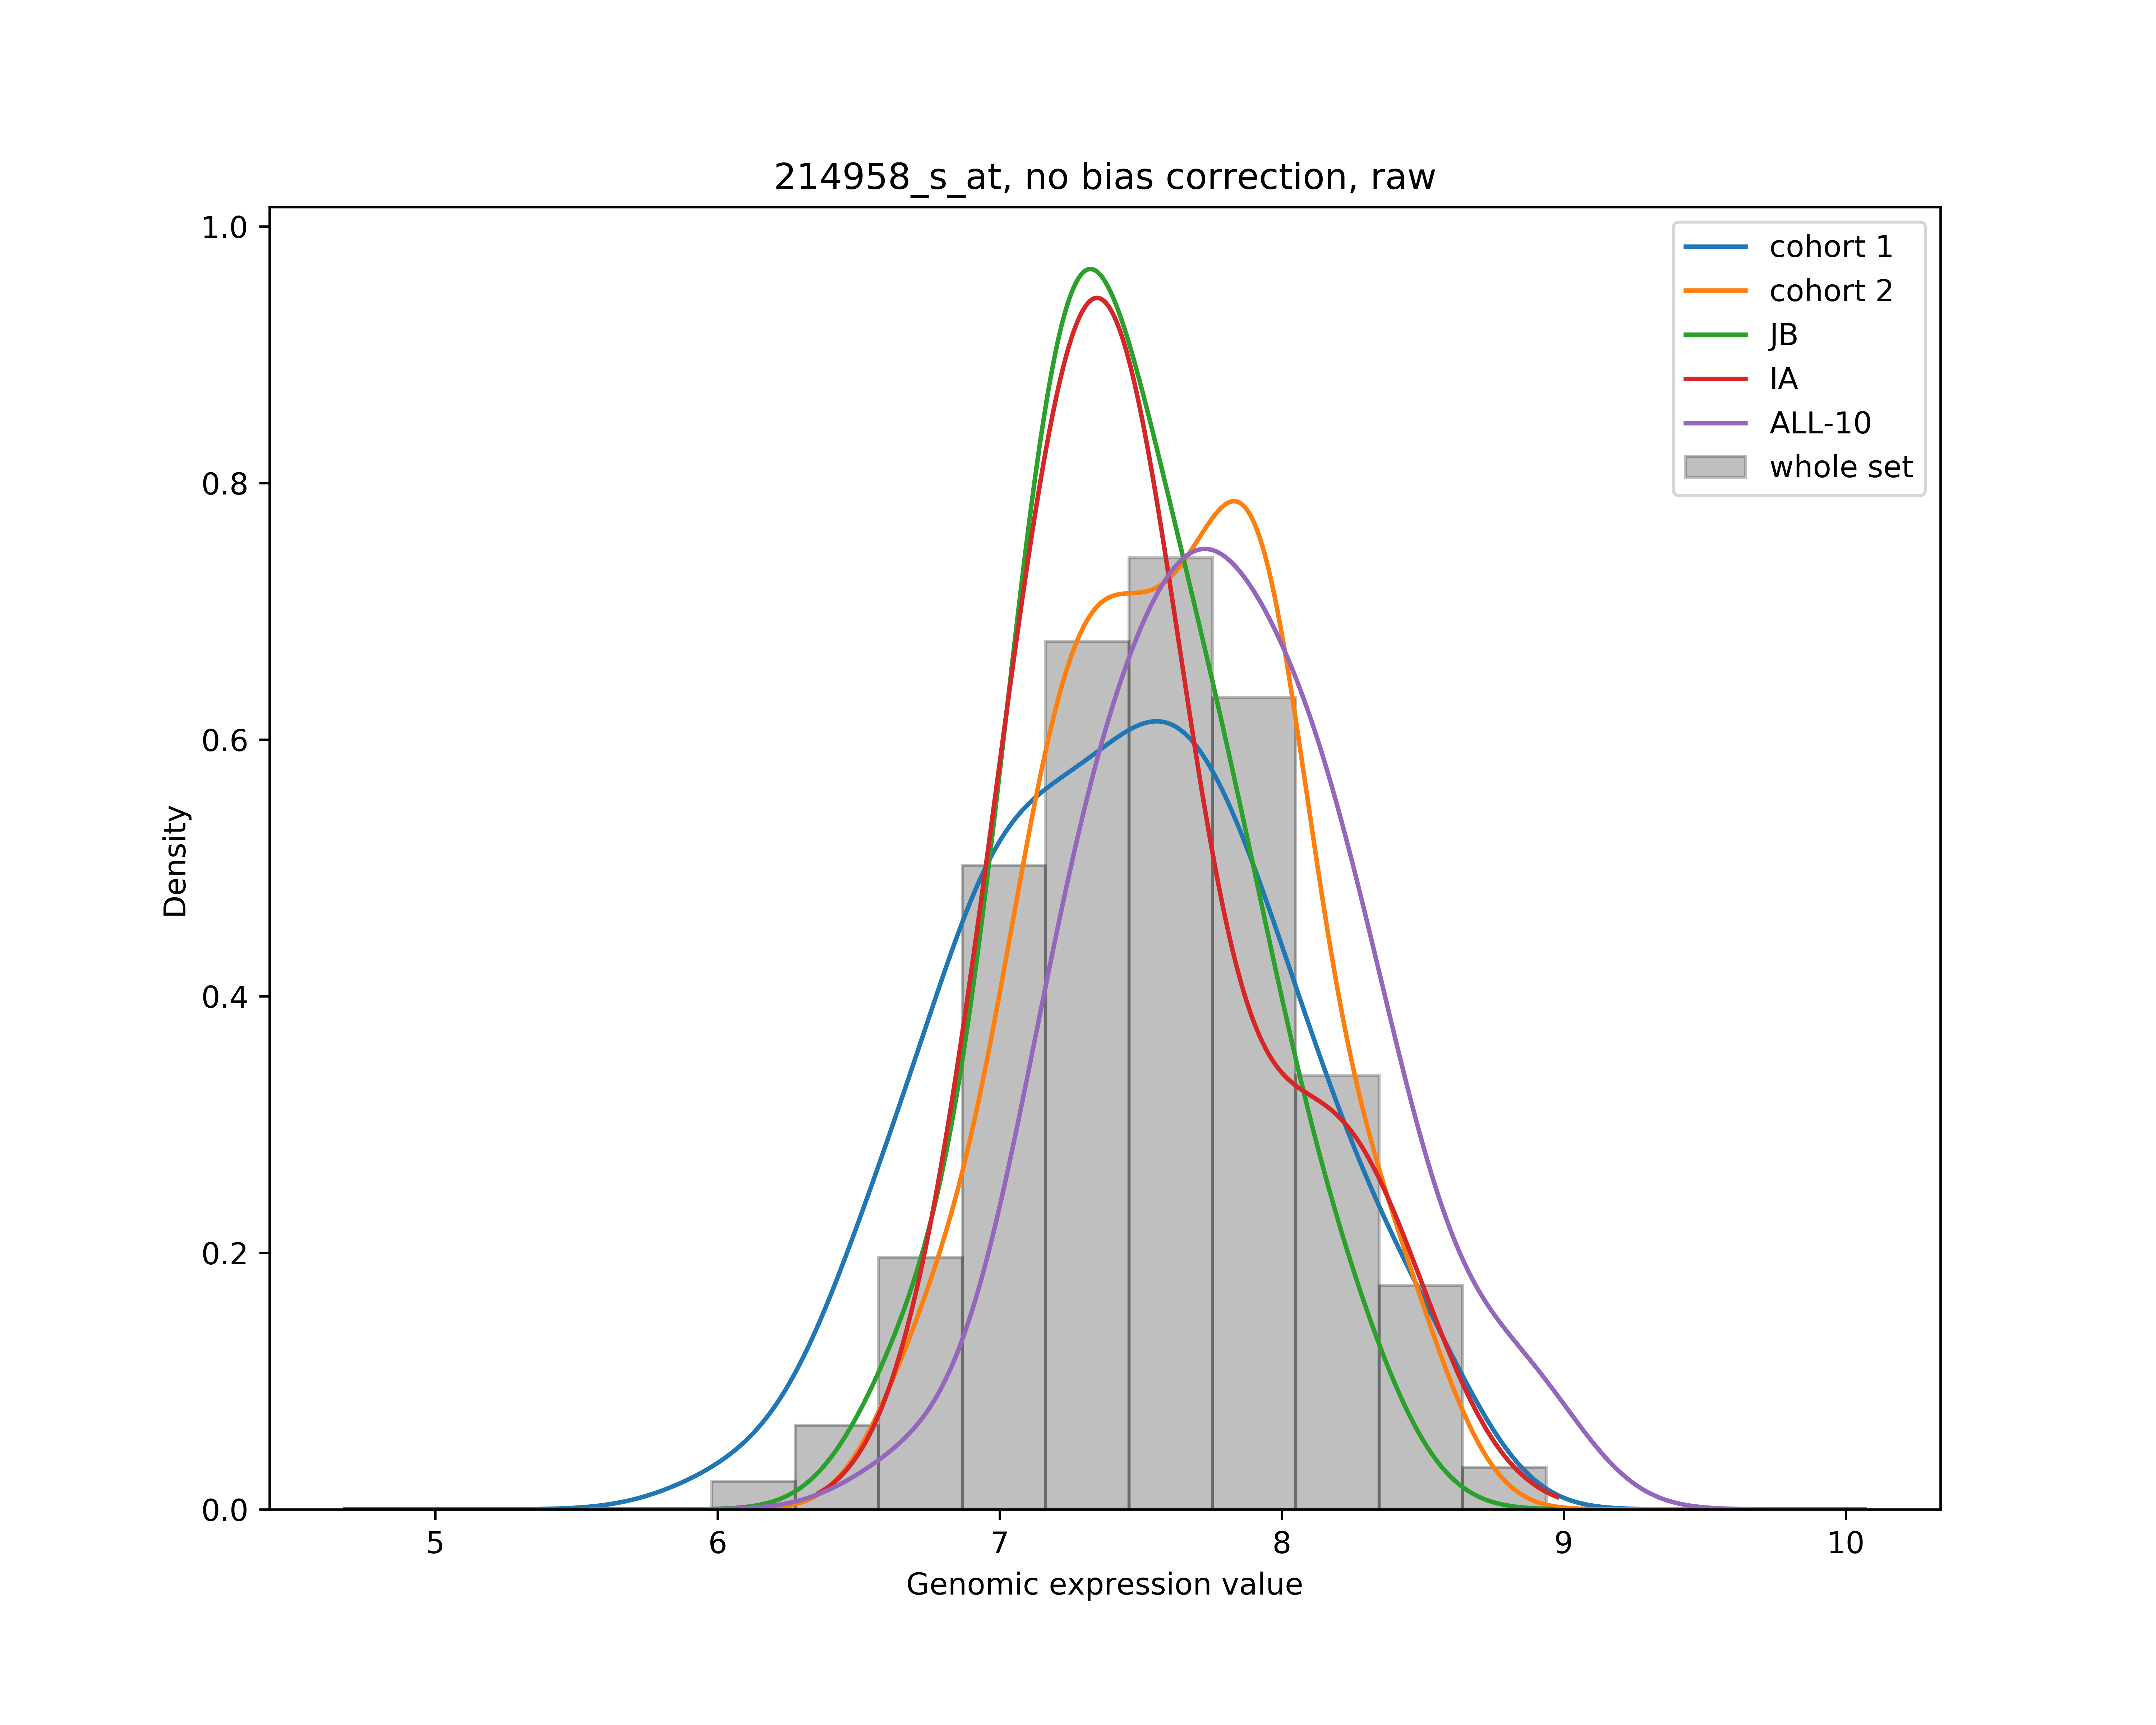
\includegraphics[width=6cm]{images/weak_genome_distribution_noCorrection_noNormalisation}
\caption{Two sets of distributions prior the bias correct, for, (left) a strong predictor and (right) a weak predictor}
\label{fig:expression_distribution_cohorts}
\end{figure}
%
\begin{figure}[htp]
\centering
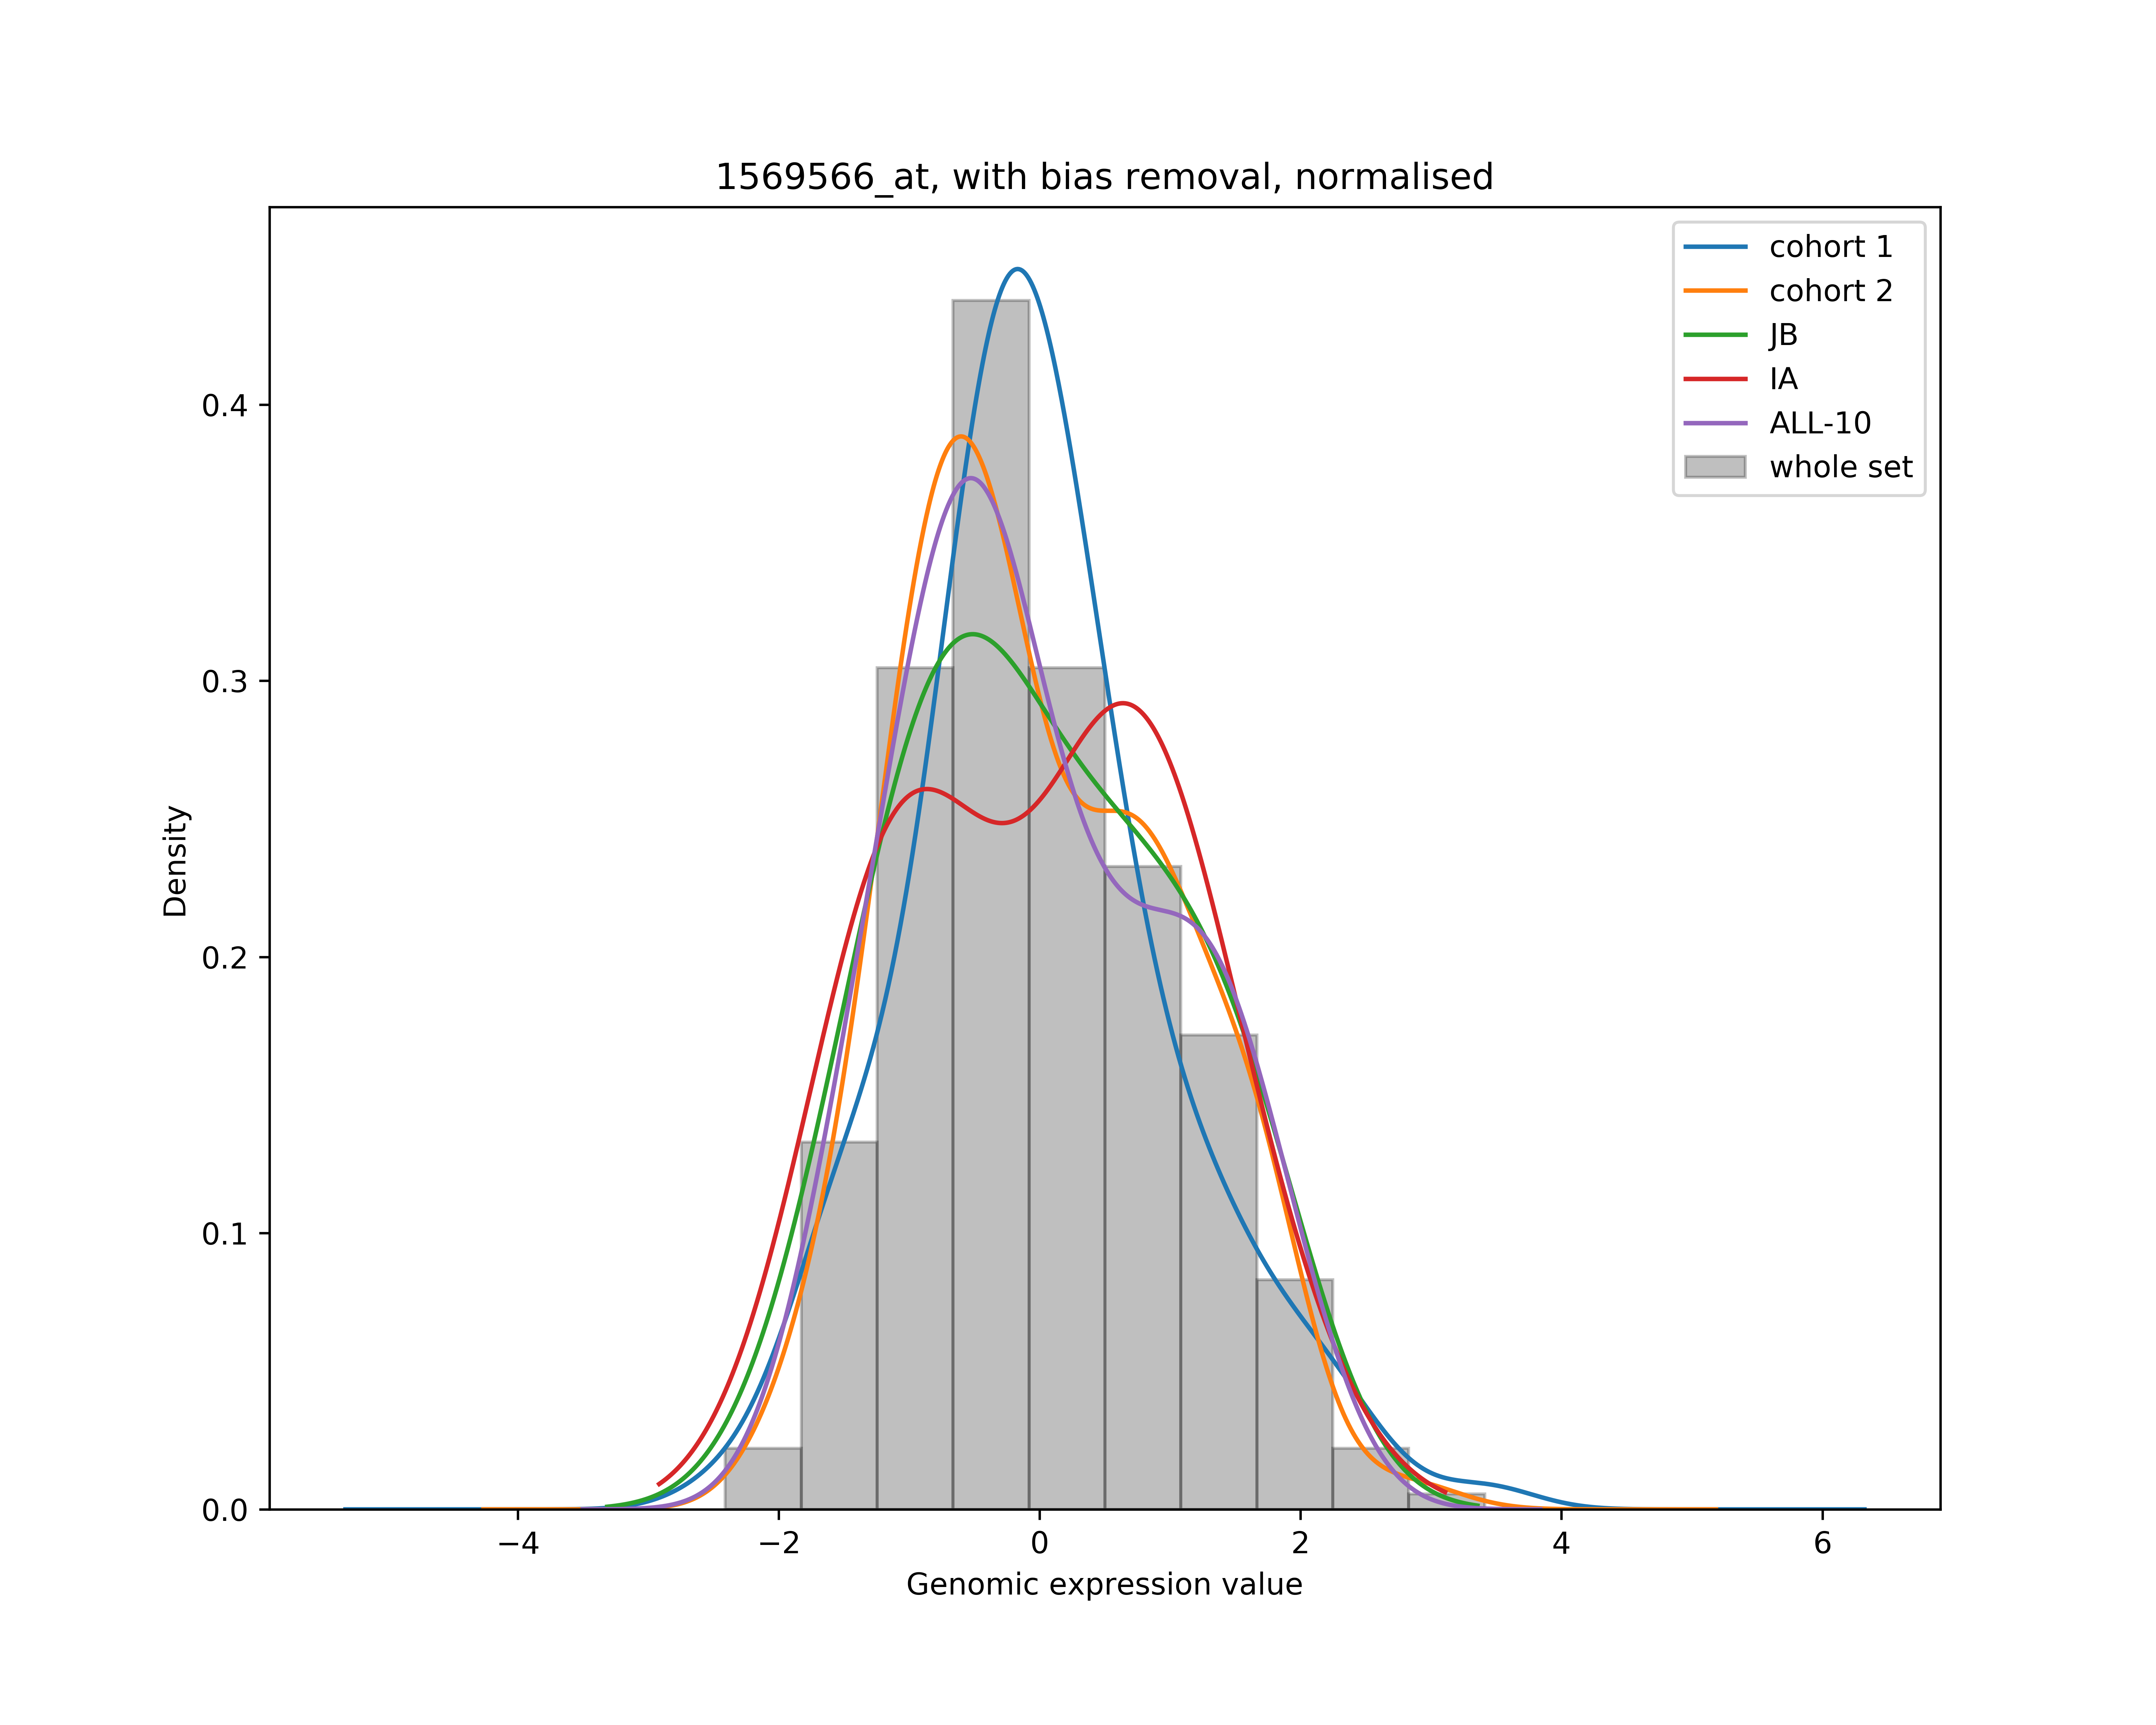
\includegraphics[width=6cm]{images/strong_genome_distribution_withCorrection_standardNormalisation}
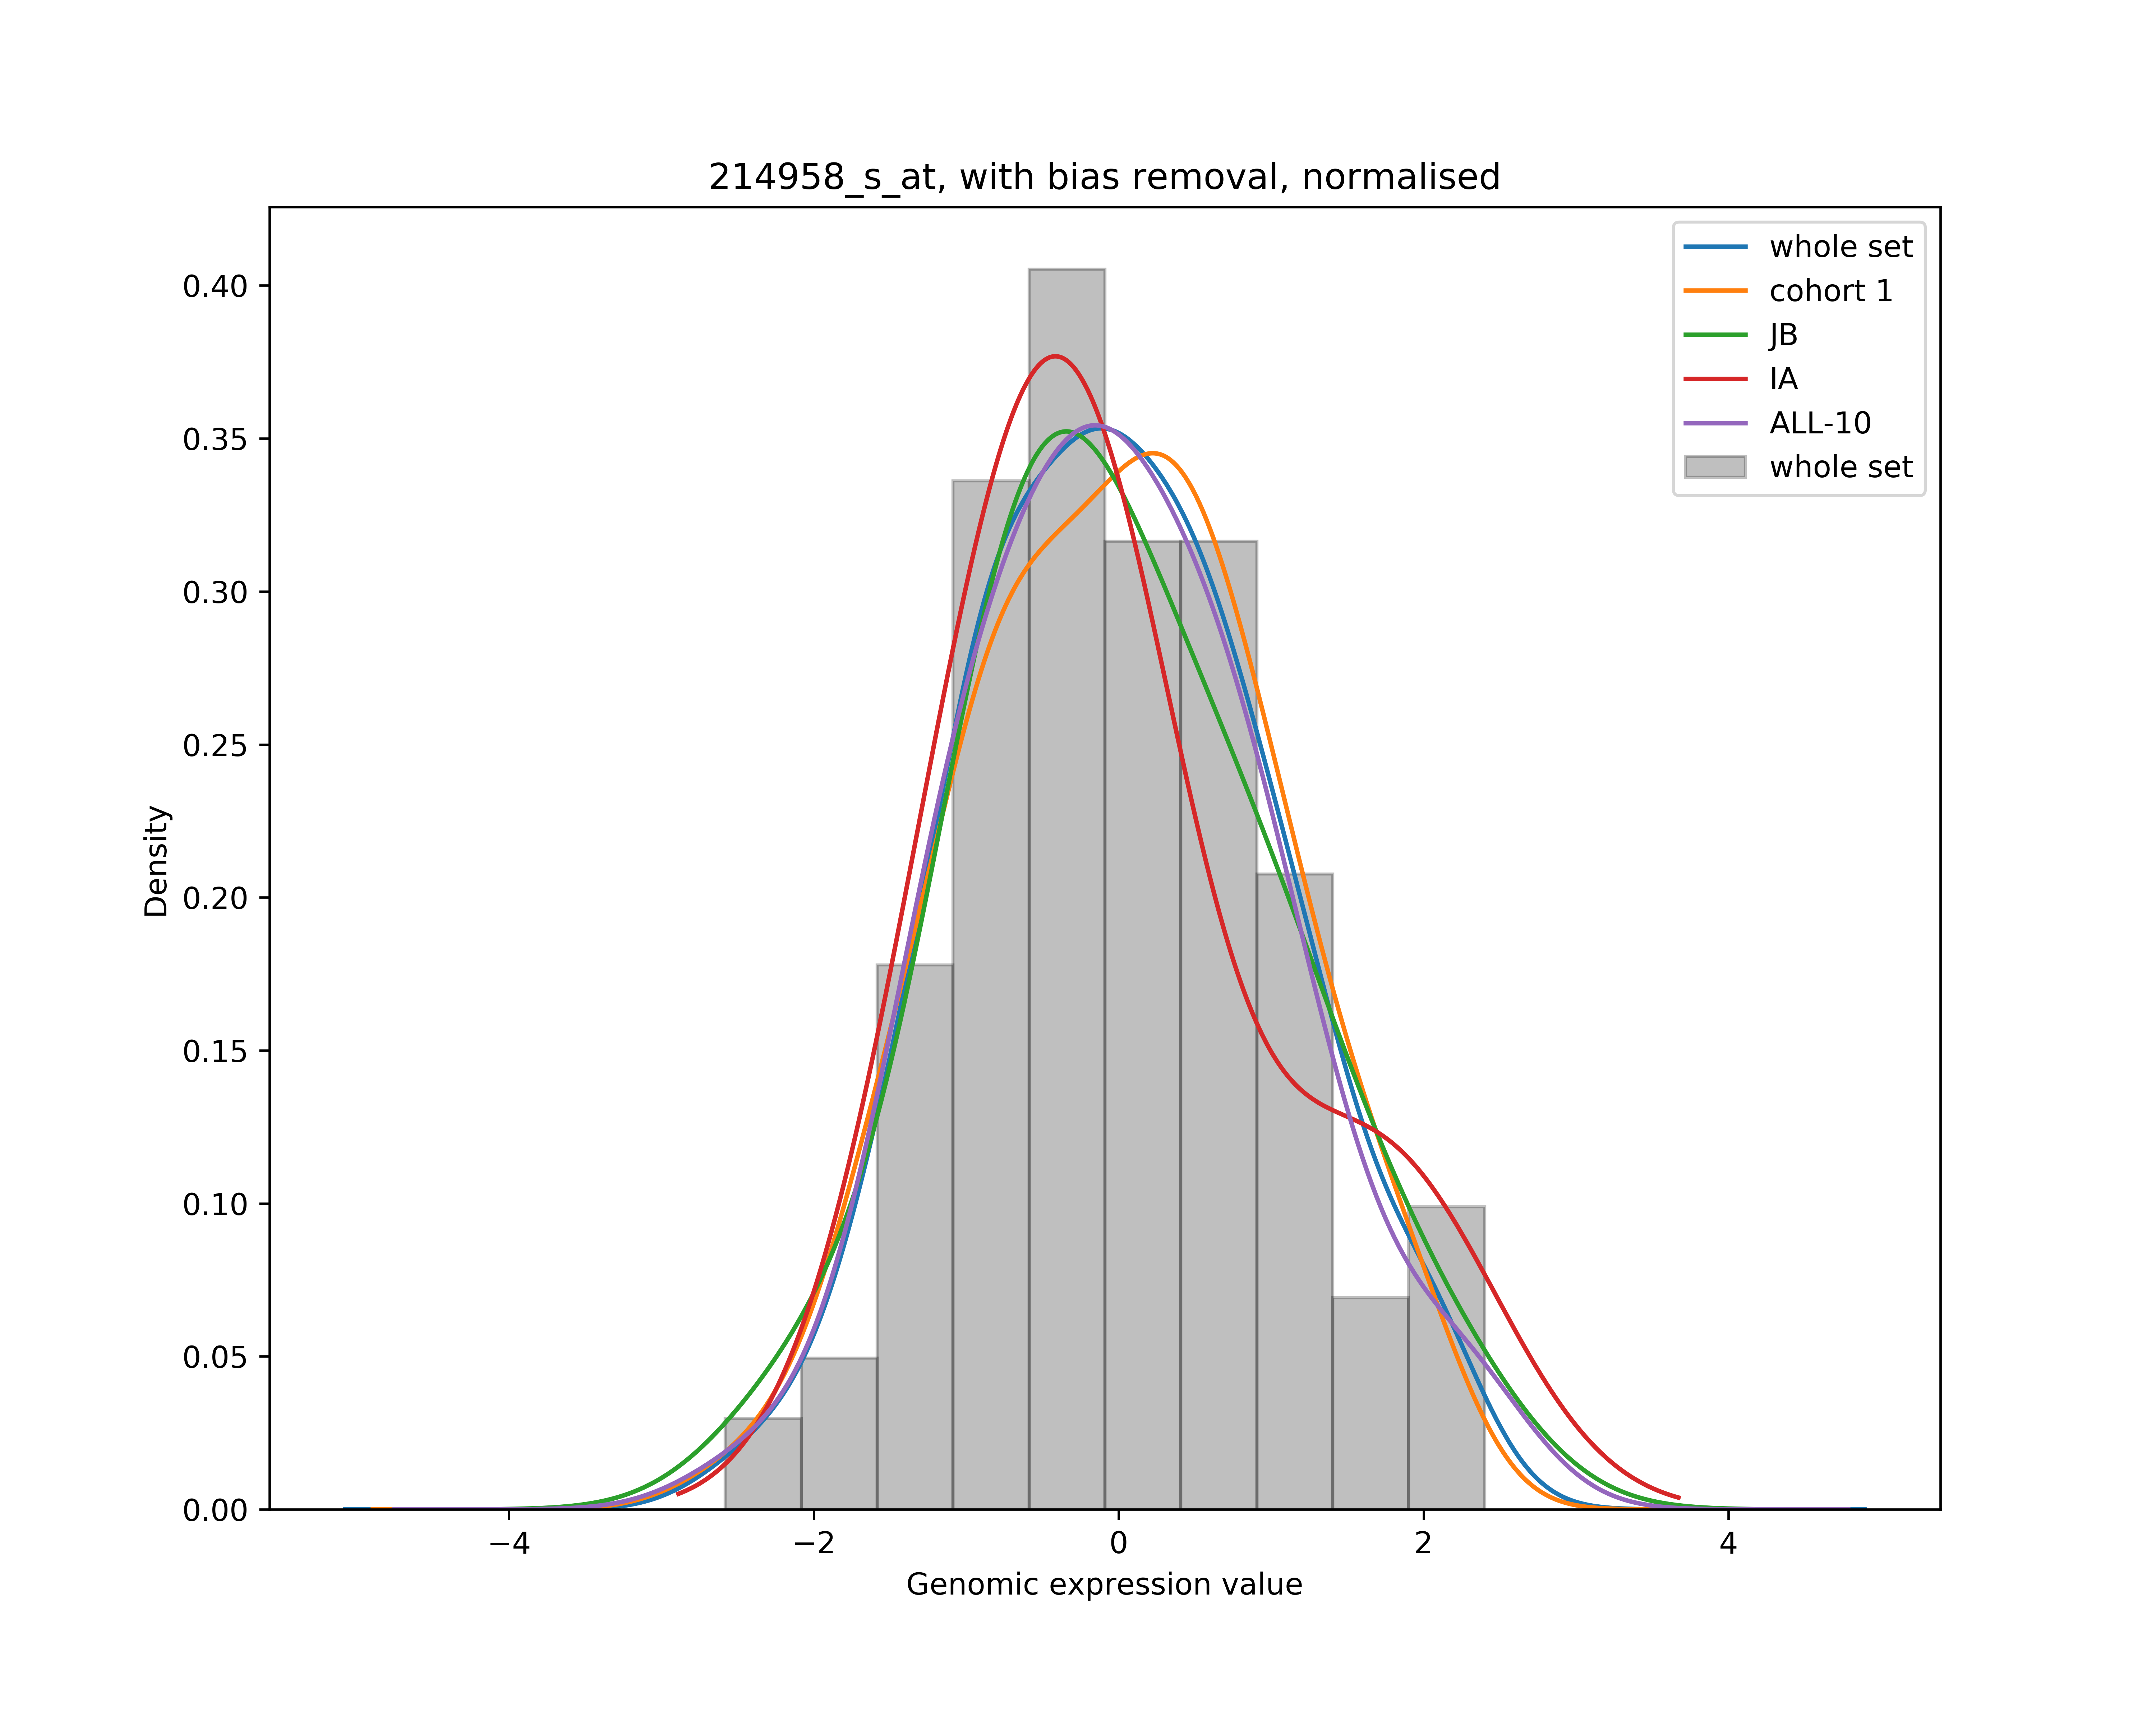
\includegraphics[width=6cm]{images/weak_genome_distribution_withCorrection_standardNormalisation}
\caption{Two sets of distributions with L/S cohort correct, for, (left) a strong predictor and (right) a weak predictor}
\label{fig:expression_distribution_cohorts_withBiasCorrection}
\end{figure}
%Strong: 1569566_at, 223748_at, 223017_at, 1568713_a_at, 201015_s_at
%Weak: 214958_s_at, 200934_at, 207908_at, 205107_s_at, 243806_at
%
There are various more elaborate methods to remove bias such as the SVD-based method from Alter et al.\cite{Alter2000}, the 
PCA-based bias removal methods EIGENSTRAT by Price et al.\cite{Price2006}, MANCIE by Zang et al.\cite{Zang2016}, the distance weighted discrimination (DWD)
approach from Benito et al.\cite{Benito2005} or the ComBat method by Johnson et al.\cite{Johnson2007} who apply an empirical Bayes approach. 
A comparison of bias removal methods is out of scope for this work, for more details we refer the reader to Johnson et al\cite{Johnson2007}.
The basic underlying assumption for all methods is that the samples are stratified over the cohorts, i.e. that in terms
of patients each cohort represents a random selection from the total set of patients. Also, it is assumed that 
the distribution has only one mode.

\subsection{Dimension reduction}
\subsubsection{Covariance based transformation}

%Partial least squares: overfitting

Principle Component Analysis (PCA): transformation of the feature space based on the eigenvectors 
of the covariance matrix. Can be applied to the entire dataset.  The downside is that we obfuscate the 
biological meaning of the features: any value in the feature set of the transformed matrix is now a linear combination 
of $N$ genome expression values, where $N$ is the number of dimensions. 
Linear Discrimination Analysis: requires availability of classification for fitting, hence
the transformation is biased to the training set, also the features are obfuscated similar to PCA. \\
Because the Covariance based transformation obfuscates the biological meaning of the feature vectors 
we choose variance-based feature reduction as the most suitable method to reduce the number of dimensions.
As for LDA, variance-based feature reduction has a bias towards the training set because it dismisses features solely
on the basis of variance across the different classifications which are obviously not available for the test set.

\subsubsection{Variance-based feature reduction}

We apply the False Discovery Rate method, with the Benjamin-Hochberg approach and the ANOVA model
to determine the F-values, with the maximum p-value set at $0.05$. % ANOVA versus Wilcoxon, Mann-Whitney U
%
\section{Classification}
%
We will shortly describe the methods used for the predictions and the determination of genome importances.
We will not go in detail on the selection of the method parameters, we refer the reader to the appendix for 
parameter selection.

\subsection{Tree based}

Single decision trees are known to be sensitive to changes in the input data. These ensemble methods 
help to decrease the variance without increasing the bias, i.e. increasing the ability to be generalised.
We employ several tree-ensemble methods: Random Forest (RF) by Breiman\cite{Breiman2001}, ExtraTrees (ET) by Geurts et al.\cite{Geurts2006} 
XGBoost (XGB) by Chen and Guestrin\cite{Chen2016} and (Light)GBM (LGBM) by Ke et al.\cite{Ke2017}.
The RF and ET methods are ensemble methods that combine an arbitrary number of decision trees, using bootstrapped samples,
random feature selection and a majority vote classification. The XGB and LGBM methods are ensemble methods 
that apply a technique called gradient boosting by Breiman\cite{Breiman1997}.
%
\subsection{Neural networks}

We use $2$ types of neural networks, a Deep Neural Network (DNN) and a Convolutional Neural Network (CNN). 

\subsection{Linear methods}

Logistic Regression (LR), linear Support Vector Machines (lSVM), linear discriminant analysis (LDA)

Simplicity, transparancy.

\subsection{Probabilistic methods}
%
Naive Bayes (NB), Gaussian Processes (GPC), Relevance Vector Machines (RVM)


% 
\begin{table}[htp]
\centering
\caption{Mean accuracies over $10$ runs with $1\%$ added random noise per run}
\label{tab:diversitymetrics}
\begin{tabular}{lllllll}
				& RF     & DNN 		& CNN  		& LSVM 		& 	XGB 	& 	LDA  \\
FDR $\alpha=0.05$		& 0.38   &  0.29      	&  0.38     	&  0.43    	& 0.25    	& 0.42  \\
FDR $\alpha=0.1$ 		& 1.59   &  1.70      	&  1.68 	&  1.65    	& 1.79    	& 1.66  \\
PCA $N=200$    			& 1.86   &  2.10      	&  1.88         &  1.79    	& 1.88          & 1.76  \\
LDA $N=200$        		& 1.54   &  1.73      	&  1.65         &  1.56    	& 1.48          & 1.55  \\
PCA $N=500$    			& 1.86   &  2.10      	&  1.88         &  1.79    	& 1.88          & 1.76  \\
LDA $N=500$        		& 1.54   &  1.73      	&  1.65         &  1.56    	& 1.48          & 1.55  \\
\end{tabular}
\end{table}
%

The tree-methods are not sensitive to the bias removal, or to the normalisation.

\section{Post-processing}
%
Description of weight/importance retrieval

\section{Discussion}

\begin{itemize}
\item if we choose PCA, LDA, check for inflection point in eigenvalue magnitude to 'smartly' select the number of components
\item successively apply standard scaling and maxabs scaling to center cohort data?
\item improve bias removal method L/S by ignoring outliers during normalisation
\item we can combine the different models in one meta-model. This bagging of models increases the accuracy, removes method-specific biases and at the same time its helps reduce overfitting.
The downside of bagging is that it obfuscates the results.
\end{itemize}

\bibliographystyle{plain}
\bibliography{methods}
\end{document}
